% Author: Zhang Rui
\documentclass[border=3pt,tikz]{standalone}
\usepackage{amsmath} % for aligned
\usepackage{listofitems} % for \readlist to create arrays
\usetikzlibrary{arrows.meta} % for arrow size
\usepackage[outline]{contour} % glow around text
\contourlength{1.4pt}

% COLORS
\usepackage{xcolor}
\colorlet{myred}{red!80!black}
\colorlet{myblue}{blue!80!black}
\colorlet{mygreen}{green!60!black}
\colorlet{myorange}{orange!70!red!60!black}
\colorlet{mydarkred}{red!30!black}
\colorlet{mydarkblue}{blue!40!black}
\colorlet{mydarkgreen}{green!30!black}

% STYLES
\tikzset{
  >=latex, % for default LaTeX arrow head
  node/.style={thick,circle,draw=myblue,minimum size=22,inner sep=0.5,outer sep=0.6},
  node in/.style={node,green!20!black,draw=mygreen!30!black,fill=mygreen!25},
  node hidden/.style={node,blue!20!black,draw=myblue!30!black,fill=myblue!20},
  node convol/.style={node,orange!20!black,draw=myorange!30!black,fill=myorange!20},
  node out/.style={node,red!20!black,draw=myred!30!black,fill=myred!20},
  connect/.style={thick,mydarkblue}, %,line cap=round
  connect arrow/.style={-{Latex[length=4,width=3.5]},thick,mydarkblue,shorten <=0.5,shorten >=1},
  node 1/.style={node in}, % node styles, numbered for easy mapping with \nstyle
  node 2/.style={node hidden},
  node 3/.style={node out}
}
\def\nstyle{int(\lay<\Nnodlen?min(2,\lay):3)} % map layer number onto 1, 2, or 3

\begin{document}

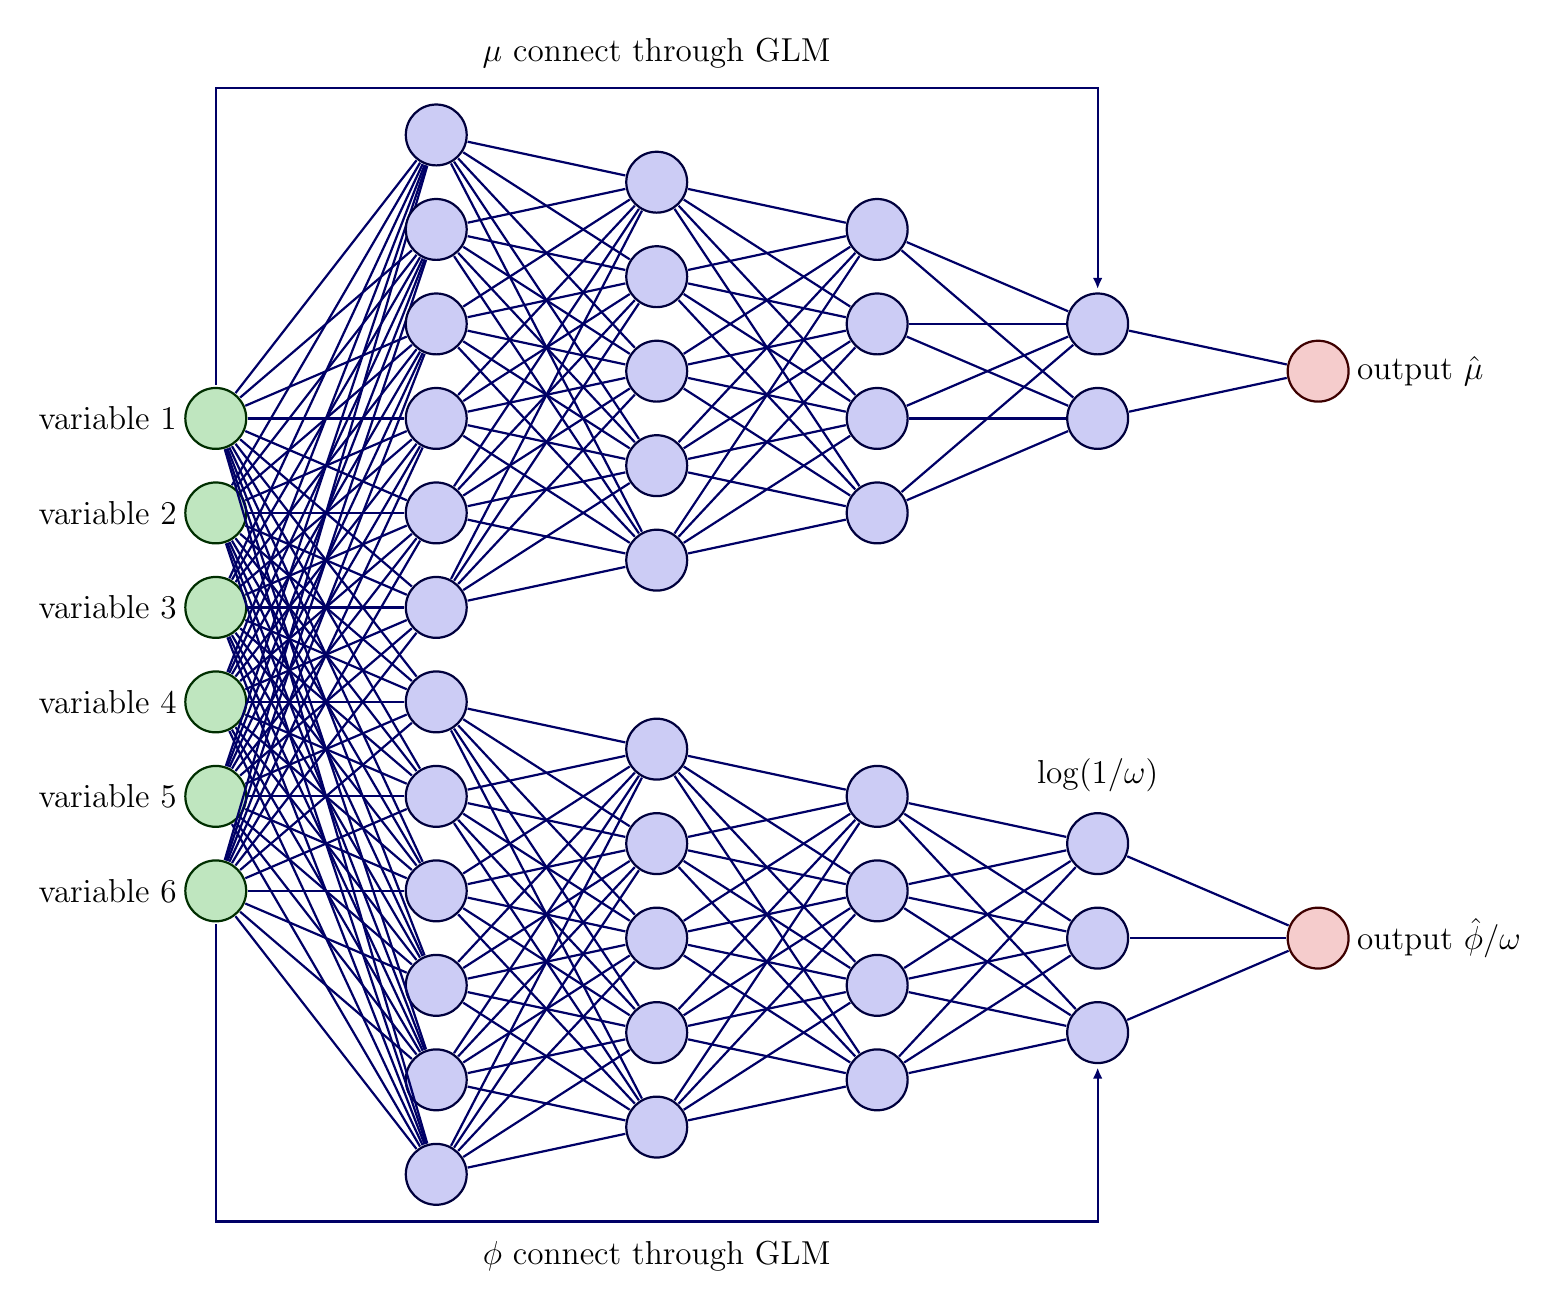
\begin{tikzpicture}[x=2.8cm,y=1.2cm]
  \large
  \message{^^JNeural network without arrows}
  \readlist\Nnod{6,12,10,8,5,2} % array of number of nodes per layer
  
  \message{^^J  Layer}
  \foreachitem \N \in \Nnod{ % loop over layers
    \def\lay{\Ncnt} % alias of index of current layer
    \pgfmathsetmacro\prev{int(\Ncnt-1)} % number of previous layer
    \message{\lay,}
    \foreach \i in {1,...,\N}{
      \pgfmathsetmacro\x{\lay}
      \pgfmathsetmacro\n{\nstyle}
      \pgfmathsetmacro\y{\N/2-\i+0.5}
      \pgfmathsetmacro\m{\N/2+1}
      \pgfmathsetmacro{\yu}{\y+(\lay-2)/2}
      \pgfmathsetmacro{\yd}{\y-(\lay-2)/2}
      \pgfmathsetmacro{\ydd}{\yd-0.5}
      \pgfmathsetmacro{\yuuu}{\yu+0.5}
      
      % NODES
      \ifnum\lay=5
        \ifnum\i<3
            \node[node \n,outer sep=0.6] (N\lay-\i) at (\x,\yu) {};
        \else
            \node[node \n,outer sep=0.6] (N\lay-\i) at (\x,\ydd) {};
        \fi
      \else
        \ifnum\lay>2
            \ifnum\lay<6
                \ifnum\i<\m
                    \node[node \n,outer sep=0.6] (N\lay-\i) at (\x,\yu) {};
                \else
                    \node[node \n,outer sep=0.6] (N\lay-\i) at (\x,\yd) {};
                \fi
            \else
                \ifnum\i=1
                    \node[node \n,outer sep=0.6] (N\lay-\i) at (\x,\yuuu) {};
                \else
                    \node[node \n,outer sep=0.6] (N\lay-\i) at (\x,\ydd) {};
                \fi
            \fi
        \else
            \node[node \n,outer sep=0.6] (N\lay-\i) at (\x,\y) {};
        \fi
      \fi
      
      % CONNECTIONS
      \ifnum\lay=2
            \foreach\j in {1,2,3,4,5,6}{
                \draw[connect] (N\prev-\j) -- (N\lay-\i);}
      \fi
      
      \ifnum\lay=3
        \ifnum\i<6
            \foreach\j in {1,2,3,4,5,6}{
                \draw[connect] (N\prev-\j) -- (N\lay-\i);}
        \else
            \foreach\j in {7,8,9,10,11,12}{
                \draw[connect] (N\prev-\j) -- (N\lay-\i);}
        \fi
      \fi

      \ifnum\lay=4
        \ifnum\i<5
            \foreach\j in {1,2,3,4,5}{
                \draw[connect] (N\prev-\j) -- (N\lay-\i);}
        \else
            \foreach\j in {6,7,8,9,10}{
                \draw[connect] (N\prev-\j) -- (N\lay-\i);}
        \fi
      \fi

      \ifnum\lay=5
        \ifnum\i<3
            \foreach\j in {1,2,3,4}{
                \draw[connect] (N\prev-\j) -- (N\lay-\i);}
        \else
            \foreach\j in {5,6,7,8}{
                \draw[connect] (N\prev-\j) -- (N\lay-\i);}
        \fi
      \fi

      \ifnum\lay=6
        \ifnum\i=1
            \foreach\j in {1,2}{
                \draw[connect] (N\prev-\j) -- (N\lay-\i);}
        \else
            \foreach\j in {3,4,5}{
                \draw[connect] (N\prev-\j) -- (N\lay-\i);}
        \fi
      \fi
    }
  }
  
  \draw[connect arrow] (N1-1) |- (3.5,6) -| (N5-1);
  \draw[connect arrow] (N1-6) |- (3.5,-6) -| (N5-5);

  % LABELS
  % \node[above=5,align=center,mygreen!60!black] at (N1-1.90) {input\\[-0.2em]layer};
  % \node[above=2,align=center,myblue!60!black] at (N3-1.90) {hidden layers};
  % \node[above=8,align=center,myred!60!black] at (N\Nnodlen-1.90) {output\\[-0.2em]layer};

  \node[left=10,align=center,black] at (N1-1) {variable 1};
  \node[left=10,align=center,black] at (N1-2) {variable 2};
  \node[left=10,align=center,black] at (N1-3) {variable 3};
  \node[left=10,align=center,black] at (N1-4) {variable 4};
  \node[left=10,align=center,black] at (N1-5) {variable 5};
  \node[left=10,align=center,black] at (N1-6) {variable 6};

  \node[above=3,align=center,black] at (N5-3.90) {$\log(1/\omega)$};

  \node[above=3,align=center,black] at (3,6) {$\mu$ connect through GLM};
  \node[below=3,align=center,black] at (3,-6) {$\phi$ connect through GLM};

  \node[right=10,align=center,black] at (N6-1) {output $\hat{\mu}$};
  \node[right=10,align=center,black] at (N6-2) {output $\hat{\phi}/\omega$};



\end{tikzpicture}




\end{document}